\chapter{Vyhodnotenie navrhovaného riešenia}\label{ch:vyhodnotenie-navrhovaneho-riesenia}

Primárnym výsledkom nášho navrhovaného riešenia bolo zabezpečenie prístupu na vzdialené zariadenie.
Samotný prístup na koncové zariadenia musí spĺňať bezpečnostné požiadavky vo všetkých fázach implementovaného prípadu
použitia.
Ďalším dôležitým cieľom bolo zaistenie komunikácie medzi jednotlivými časťami systému a modulárne navrhnúť všetky potrebné
súčasti tak, aby ich bolo možné s pribúdajúcimi kritériami bezpečnosti, alebo použitia jednoducho doimplementovať.

Pri nasadení nášho riešenia, v systéme figuruje iba používateľ typu „superuser“, ktorý má všetky systémové práva.
Tento používateľ vie vytvoriť potrebné záznamy, ako napríklad: projekty, koncové zariadenia, role, používateľov, a ďalšie,
ktoré sú nevyhnutné pre správne fungovanie systému.

Vytvorenie používateľa s rolou „devops“ je po prihlásení superuserom nasledovné:
\newpage
\textbf{\large Požiadavka [POST]:}

\begin{lstlisting}[language=json,firstnumber=1]
{
  "email": "devops@praetorian.sk",
  "password": "devops",
  "name": "devops",
  "surname": "devops",
  "role": "devops",
  "is_vpn": false,
  "additional_data": {},
  "language_id": "ee3f8e7a-c9d8-4d96-8dd0-816775b25b7d"
}
\end{lstlisting}

\textbf{\large Odpoveď:}

\begin{lstlisting}[language=json,firstnumber=1]
{
  "response": {
    "id": "dbab895b-5568-45bf-95a3-55d96118836c",
    "username": "devops@praetorian.sk",
    "name": "devops",
    "surname": "devops",
    "email": "devops@praetorian.sk",
    "phone": null,
    "role": "devops",
    "is_temporary": false,
    "additional_data": {}
  }
}
\end{lstlisting}

Po úspešnom vytvorení používateľa a po registrovaní jeho zariadenia v systéme, je mu možné priradiť superuserom jeden z
existujúcich projektov v systéme a následne sa za neho prihlásiť:

\textbf{\large Požiadavka [POST]:}

\begin{lstlisting}[language=json,firstnumber=1]
{
  "username": "devops@praetorian.sk",
  "password": "devops"
}
\end{lstlisting}

\textbf{\large Odpoveď:}

\begin{lstlisting}[language=json,firstnumber=1]
{
  "response": {
    "token": "22fcf8a5-7c90-4e3a-a665-7cf842b46283",
    "active_2fa": false
  }
}
\end{lstlisting}

Ako je z odpovede webového api rozhrania vidieť, používateľ nie je overený dvojfaktorovou autentifikáciou.
Táto hodnota sa v odpovedi nachádza z dôvodu informovania, či je potrebné vyžiadanie tohto dodatočného typu autentifikácie.

Pre vyžiadanie dvojfaktorovej autentifikácie je potrebné si danú službu aktivovať nasledovným spôsobom:

\textbf{\large Požiadavka [GET]:}

\inlinecode{\{\{ api\_url \}\}/v1/users/\{\{ user\_id \}\}/2fa/}

\newpage
\textbf{\large Odpoveď:}

\begin{lstlisting}[language=json,firstnumber=1]
{
  "response": {
    "qr_code": "otpauth://totp/Praetorian%20API:devops%40praetorian.sk?secret=J4UZONZ36IQGLZAM&issuer=Praetorian%20API"
  }
}
\end{lstlisting}

Reťazec v odpovedi slúži na vytvorenie qr kódu, ktorý bude zobrazený v grafickom užívateľskom rozhraní, pričom používateľ
je taktiež o aktivácii dvojfaktorovej autentifikácie informovaný pomocou zaslaného systémového emailu, ktorého obsah
je na obrázku~\ref{fig:obr_13}.

\begin{figure}[H]
\begin{center}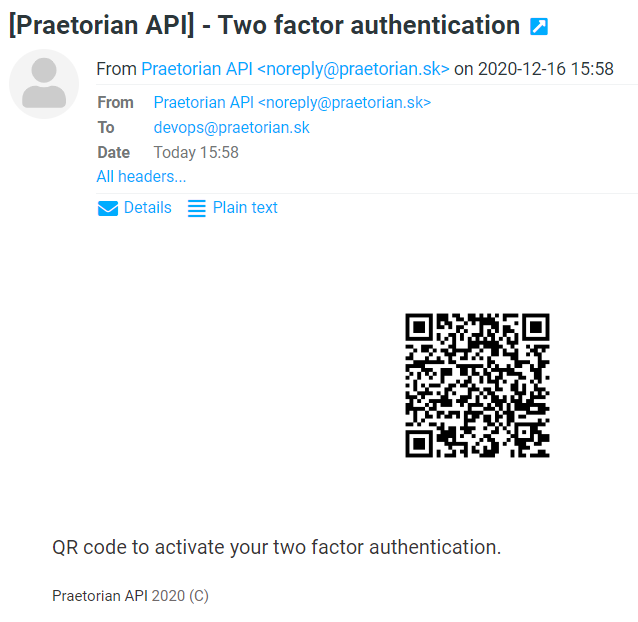
\includegraphics[width=\textwidth,height=9cm,keepaspectratio=true]{assets/2fa_email.png}\end{center}
\caption[Obsah emailu informujúcom o aktivácii dvojfaktorovej autentifikácie]{Obsah emailu informujúcom o aktivácii dvojfaktorovej autentifikácie}\label{fig:obr_14}
\end{figure}

Naskenovaním daného qr kódu, napríklad v aplikácii „Authenticator“, sa vytvorí nový účet, ktorému je priradený práve jeden OTP
s veľmi krátkou životnosťou.
Po uplynutí životnosti sa OTP automaticky pregeneruje.
Vytvorený účet v aplikácii Authenticator so zobrazeným OTP je znázornený na obrázku~\ref{fig:obr_15}.

\begin{figure}[H]
\begin{center}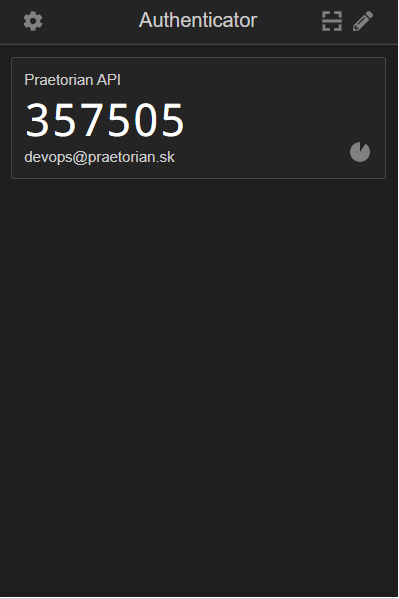
\includegraphics[width=\textwidth,height=9cm,keepaspectratio=true]{assets/authenticator.png}\end{center}
\caption[Zobrazenie aktivovaného účtu s OTP v aplikácii Authenticator]{Zobrazenie aktivovaného účtu s OTP v aplikácii Authenticator}\label{fig:obr_15}
\end{figure}

Ďalšou z možností nami vytvoreného používateľa je pripojenie sa na vzdialené zariadenie pomocou ssh proxy servera, pričom na
pripojenie je použité interaktívne prostredie.
Celý proces pripojenia používateľa ku koncovému zariadeniu je zobrazený na obrázku~\ref{fig:obr_16}

\begin{figure}[H]
\begin{center}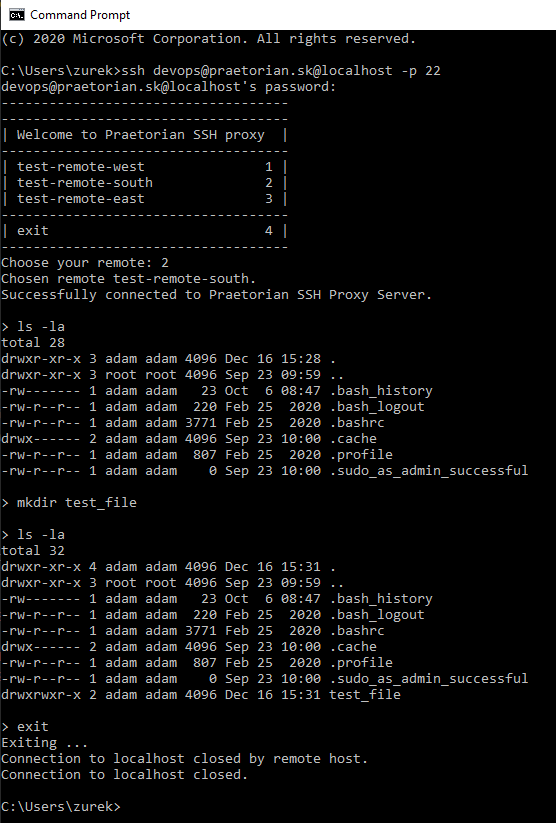
\includegraphics[width=\textwidth,height=15cm,keepaspectratio=true]{assets/interactive_session.png}\end{center}
\caption[Proces pripojenia cez interaktívne prostredie]{Proces pripojenia cez interaktívne prostredie}\label{fig:obr_16}
\end{figure}

Používateľ cez interaktívne prostredie vytvoril na koncovom zariadení priečinok s názvom „test\_file“.
Ak chce cez neinteraktívne prostredie daný priečinok zmazať, musí si v prvom rade vytvoriť skript, ktorý bude obsahovať
tri príkazy:
\newpage

\begin{enumerate}
  \item \inlinecode{ls -la}
  \item \inlinecode{rmdir log\_entries}
  \item \inlinecode{ls -la}
\end{enumerate}

Nasledovne si musí vytvoriť dočasného používateľa, ktorého úlohou bude daný skript jednorázovo vykonať, pričom bude po
dokončení úlohy dočasný požívateľ vymazaný.
Pre vytvorenie dočasného používateľa je potrebné sa prihlásiť za permanentného používateľa do webového api rozhrania a
vytvoriť nasledovnú požiadavku:

\textbf{\large Požiadavka [POST]:}

\begin{lstlisting}[language=json,firstnumber=1]
{
  "project_id": "408c57f3-6ea4-42dc-beb3-a0051b97182f",
  "remote_id": "f2228baf-d999-4d7a-9780-b8f2be97956f"
}
\end{lstlisting}

\textbf{\large Odpoveď:}

\begin{lstlisting}[language=json,firstnumber=1]
{
  "response": {
    "username": "jPTgEYC@praetorian.sk",
    "password": "AnVV6kLPA9"
  }
}
\end{lstlisting}

Používateľovi taktiež v prípade zabudnutia prístupových údajov k dočasnému používateľovi dôjde notifikácia s potrebnými
informáciami, ktorej obsah je zobrazený na obrázku~\ref{fig:obr_17}.

\begin{figure}[H]
\begin{center}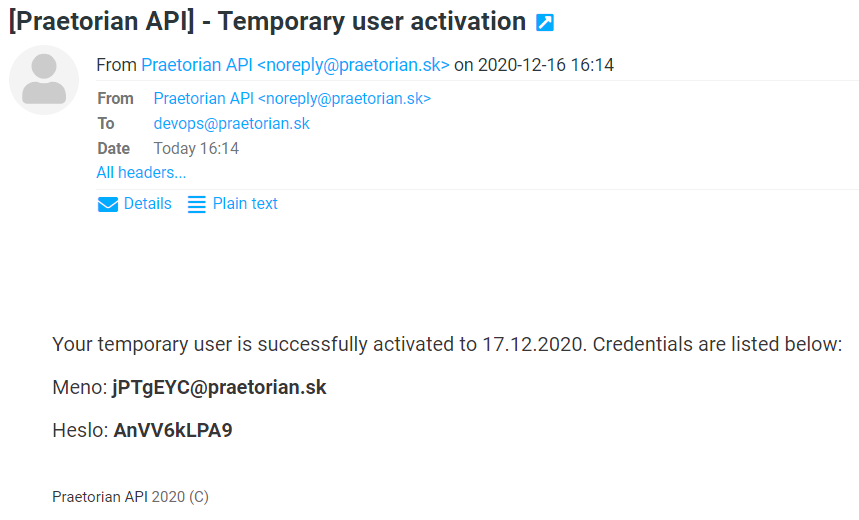
\includegraphics[width=\textwidth,height=9cm,keepaspectratio=true]{assets/temporary_credentials.png}\end{center}
\caption[Obsah emailu informujúcom o prístupových údajoch dočasného používateľa]{Obsah emailu informujúcom o prístupových údajoch dočasného používateľa}\label{fig:obr_17}
\end{figure}

Po úspešnom vytvorení skriptu a dočasného používateľa je možné sa pripojiť na koncové zariadenie cez neinteraktívne prostredie,
ktorého vykonanie je na obrázku~\ref{fig:obr_18}.

\begin{figure}[H]
\begin{center}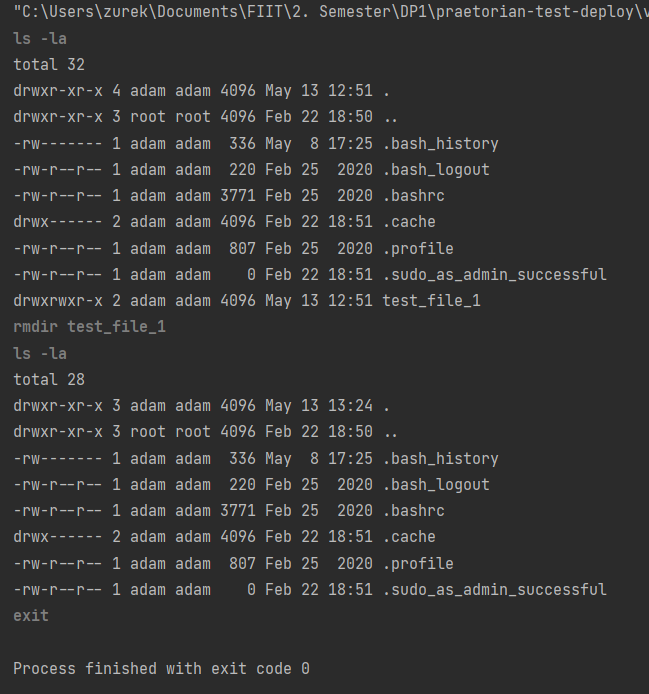
\includegraphics[width=\textwidth,height=12cm,keepaspectratio=true]{assets/non_interactive_session.png}\end{center}
\caption[Proces pripojenia cez neinteraktívne prostredie]{Proces pripojenia cez neinteraktívne prostredie}\label{fig:obr_18}
\end{figure}

Po úspešnom dokončení vykonávania príkazov na dané koncové zariadenie, bolo nasledovne ukončené spojenie a dočasný používateľ
bol vymazaný.

Dané riešenie pokrýva viacero scenárov použitia, ako napríklad manažment používateľov, projektov a skupín, monitorovanie
všetkých systémových akcií, kontrola povolených zariadení a mnoho ďalších.
No hlavnou úlohou v danej fáze riešenia bolo predovšetkým preukázať zmysel riešeného zadania preukázanou modularitou a procesom
bezpečného pripojenia na vzdialené zariadenia, ktorý je možné rozširovať o nové bezpečnostné prvky a prípady použitia.
